% Für Bindekorrektur als optionales Argument "BCORfaktormitmaßeinheit", dann
% sieht auch Option "twoside" vernünftig aus
% Näheres zu "scrartcl" bzw. "scrreprt" und "scrbook" siehe KOMA-Skript Doku
\documentclass[12pt,a4paper,titlepage,headinclude,bibtotoc]{scrartcl}


%---- Allgemeine Layout Einstellungen ------------------------------------------

% Für Kopf und Fußzeilen, siehe auch KOMA-Skript Doku
\usepackage[komastyle]{scrpage2}
\pagestyle{scrheadings}
\setheadsepline{0.5pt}[\color{black}]
\automark[section]{chapter}


%Einstellungen für Figuren- und Tabellenbeschriftungen
\setkomafont{captionlabel}{\sffamily\bfseries}
\setcapindent{0em}


%---- Weitere Pakete -----------------------------------------------------------
% Die Pakete sind alle in der TeX Live Distribution enthalten. Wichtige Adressen
% www.ctan.org, www.dante.de

% Sprachunterstützung
\usepackage[ngerman]{babel}

% Benutzung von Umlauten direkt im Text
% entweder "latin1" oder "utf8"
\usepackage[utf8]{inputenc}

% Pakete mit Mathesymbolen und zur Beseitigung von Schwächen der Mathe-Umgebung
\usepackage{latexsym,exscale,stmaryrd,amssymb,amsmath}

% Weitere Symbole
\usepackage[nointegrals]{wasysym}
\usepackage{eurosym}

% Anderes Literaturverzeichnisformat
%\usepackage[square,sort&compress]{natbib}

% Für Farbe
\usepackage{color}

% Zur Graphikausgabe
%Beipiel: \includegraphics[width=\textwidth]{grafik.png}
\usepackage{graphicx}

% Text umfließt Graphiken und Tabellen
% Beispiel:
% \begin{wrapfigure}[Zeilenanzahl]{"l" oder "r"}{breite}
%   \centering
%   \includegraphics[width=...]{grafik}
%   \caption{Beschriftung} 
%   \label{fig:grafik}
% \end{wrapfigure}
\usepackage{wrapfig}

% Mehrere Abbildungen nebeneinander
% Beispiel:
% \begin{figure}[htb]
%   \centering
%   \subfigure[Beschriftung 1\label{fig:label1}]
%   {\includegraphics[width=0.49\textwidth]{grafik1}}
%   \hfill
%   \subfigure[Beschriftung 2\label{fig:label2}]
%   {\includegraphics[width=0.49\textwidth]{grafik2}}
%   \caption{Beschriftung allgemein}
%   \label{fig:label-gesamt}
% \end{figure}
\usepackage{subfigure}

% Caption neben Abbildung
% Beispiel:
% \sidecaptionvpos{figure}{"c" oder "t" oder "b"}
% \begin{SCfigure}[rel. Breite (normalerweise = 1)][hbt]
%   \centering
%   \includegraphics[width=0.5\textwidth]{grafik.png}
%   \caption{Beschreibung}
%   \label{fig:}
% \end{SCfigure}
\usepackage{sidecap}

% Befehl für "Entspricht"-Zeichen
\newcommand{\corresponds}{\ensuremath{\mathrel{\widehat{=}}}}
% Befehl für Errorfunction
\newcommand{\erf}[1]{\text{ erf}\ensuremath{\left( #1 \right)}}

%Fußnoten zwingend auf diese Seite setzen
\interfootnotelinepenalty=1000

%Für chemische Formeln (von www.dante.de)
%% Anpassung an LaTeX(2e) von Bernd Raichle
\makeatletter
\DeclareRobustCommand{\chemical}[1]{%
  {\(\m@th
   \edef\resetfontdimens{\noexpand\)%
       \fontdimen16\textfont2=\the\fontdimen16\textfont2
       \fontdimen17\textfont2=\the\fontdimen17\textfont2\relax}%
   \fontdimen16\textfont2=2.7pt \fontdimen17\textfont2=2.7pt
   \mathrm{#1}%
   \resetfontdimens}}
\makeatother

%Honecker-Kasten mit $$\shadowbox{$xxxx$}$$
\usepackage{fancybox}
%Honeckerbox mit Mathe \begin{emphaeq}[box=\shadowbox*]{align}...\end{emphaeq}
%\usepackage{emphaeq}

%SI-Package
\usepackage{siunitx}


\parindent0pt

%Bibliography \bibliography{literatur} und \cite{gerthsen}
%\usepackage{cite}
\usepackage{babelbib}
\selectbiblanguage{ngerman}


\begin{document}

\begin{titlepage}
\centering
\textsc{\Large Anfängerpraktikum der Fakultät für
  Physik,\\[1.5ex] Universität Göttingen}

\vspace*{4.2cm}

\rule{\textwidth}{1pt}\\[0.5cm]
{\huge \bfseries
  Versuch Diffusion\\[1.5ex]
  Protokoll}\\[0.5cm]
\rule{\textwidth}{1pt}

\vspace*{3cm}

\begin{Large}
\begin{tabular}{ll}
Praktikant: &  Michael Lohmann\\
% &  Felix Kurtz\\
Mitpraktikant: &  Kevin Lüdemann\\
% &  Skrollan Detzler\\
E-Mail: & m.lohmann@stud.uni-goettingen.de\\
% &  felix.kurtz@stud.uni-goettingen.de\\
%Mitpraktikant:  &  kevin.luedemann@stud.uni-goettingen.de\\
% &  skrollan.detzler@stud.uni-goettingen.de\\
 Betreuer: & Martin Ochmann\\
 Versuchsdatum: & 30.06.2014\\
\end{tabular}
\end{Large}

\vspace*{0.8cm}

\begin{Large}
\fbox{
  \begin{minipage}[t][2.5cm][t]{6cm} 
    Note:
  \end{minipage}
}
\end{Large}

\end{titlepage}

\tableofcontents

\newpage

\section{Einleitung}
\label{sec:einleitung}
Die Diffusion (vom lateinischen diffundere 'sich ausbreiten') ist die Eigenschaft von verschiedenen Medien, sich ohne äußere Einflüsse miteinander zu vermischen, bis ein Gleichgewichtszustand erreicht ist, nur dadurch, dass sie miteinander in Kontakt stehen.
So verursacht jede räumliche Inhomogenität einer physikalischen Größe einen Ausgleichsstrom.
Bei Materie geschieht dies aufgrund der statistischen Bewegung der Teilchen, der Braunschen Molekularbewegung.
Die Diffusion ist eine sehr wichtige Eigenschaft von Teilchen, da ohne sie zum Beispiel kein Leben existieren könnte, da kein Sauerstoff in unsere Zellen transportiert werden könnte.


\section{Theorie}
\label{sec:theorie}
\subsection{Diffusion}
Hat ein Stoff eine von 0K verschiedene Temperatur, so bewegen sich die Teilchen abhängig von dieser mit einer bestimmten Durchschnittsgeschwindigkeit in verschiedene Richtungen.
Da die Teilchen gegeneinander elastisch stoßen, ändert sich in diesem Moment ihre Geschwindigkeit, sowie deren Richtung.
Die so entstehenden zufälligen Bewegungen wurden schon 1827 von Brown entdeckt \cite[S. 8]{demtroeder}.

\subsection{Ficksche Gesetze}
Die Fickschen Gesetze beschreiben die Diffusion.
Da eine Inhomogenität einer physikalischen Größe $n(\vec x,t)$ (in unserem Fall Teilchen) einen Ausgleichsstrom $\vec j(\vec x,t)$ hervorruft, der abhängig davon ist, wie groß diese an einem bestimmten Ort $\vec x$ zu einer bestimmten Zeit $t$ ist, lautet das \emph{erste Ficksche Gesetz}:
$$\shadowbox{$\vec j(\vec x,t)=-D ~ \nabla n(\vec x,t)$}$$
Hierbei ist D die Diffusionskonstante, welche festlegt, wie groß der Teilchenstrom bei gegebener Inhomogenität eines speziellen Mediums ist.
Da die Teilchenzahl erhalten bleibt, müssen mehr Teilchen ein- bzw. ausströmen, wenn sie sich verändert.
$$\frac{\partial n(\vec x,t)}{\partial t}=-\nabla\cdot \vec j(\vec x,t)$$
Setzt man die obige Gleichung nun für $\vec j$ ein, so ergibt sich das \emph{zweite Ficksche Gesetz}
$$\shadowbox{$\frac{\partial n(\vec x,t)}{\partial t}=D~\nabla^2n(\vec x,t)$}$$
Statt mit der Teilchenzahl $n$ zu rechnen, kann man ebenfalls mit der Teilchenkonzentration $c=\dfrac{n}{V}$ rechnen


\subsection{Lösung der DGL}
Die Lösung der sich aus diesen beiden Gleichungen ergebenden Differentialgleichung wird durch die Methode der Reflektion und Superposition bestimmt (Literatur: \cite[S. 11]{crank}).
Unsere gesuchte Lösung ist die für einen Zylinder, welcher für $x>0$ zu $t=0$ eine Konzentration $c=c_0$ besitzt und zur selben Zeit bei $x<0$ keine Konzentration besitzt.
Die Grenzschicht ist also bei $x=0$.
Wir beginnen mit der Suche nach einer Lösung für eine Stoffmenge $M$, welche sich zur Zeit $t=0$ nur am Ort $x=0$ befindet.\\
Aus der Gleichung
\begin{align*}
\frac{\partial c}{\partial t}&=D\nabla^2 c\\
\end{align*}
folgt ersichtlicherweise die Lösung
\begin{align}
c'&=\frac{A}{\sqrt{t}}\exp\left(-x^2/4Dt \right)\label{eq:c1}
\end{align}
mit einer Konstante A, welche an die Anfangsbedingungen angepasst wird.
Die Gesammtmenge an diffundierenden Stoff beträgt
\begin{align*}
M=\int\limits_{-\infty}^\infty c' \; dx
\end{align*}
Was durch Einsetzen von Gleichung \eqref{eq:c1} und Substitution zu dem Ergebnis
\begin{align*}
M=2A\sqrt{\pi D}
\end{align*}
führt, was umgestellt nach $A$ und in Gleichung \eqref{eq:c1} eingesetzt heißt
\begin{align*}
c'=\frac{M}{2\sqrt{\pi D}}\exp\left(-x^2/4Dt\right)\quad .
\end{align*}
Diese spezielle Lösung kann nun verwendet werden, um unsere gesuchte herzuleiten.
Da hierbei die Hälfte des Stoffes in die positive und die andere Hälfte in die negative $x$-Richtung diffundiert, kommt zu unserer Lösung ein Faktor 2 hinzu ("Reflektion").\\
Durch Superposition dieser Lösung für alle $x>0$ kommt man letztlich zu dem Ergebnis, dass
\begin{align}
c(x,t)=\frac{c_0}{2}\left[1-\erf{\frac{x}{\sqrt{4Dt}}}\right] \label{eq:c}
\end{align}
mit der Gaußschen Fehlerfunktion
\begin{align*}
\erf{y}=\frac{2}{\sqrt{\pi}}\int\limits_0^y\exp\left(-v^2\right)~dv
\end{align*}
ist.
\subsection{Wheatstonsche Brückenschaltung und Photowiederstand}
Die Wheatstonsche Brückenschaltung ist ein Bauelement, welches zur Bestimmung von Widerständen genutzt wird.
Sie baut auf dem Prinzip der Spannungsverteilung an in Reihe geschalteten Widerständen auf.
Hat man zwei bekannter Größe und einen regelbaren, so kann man mithilfe eines Volt- oder Ampèremeters einen unbekannten vermessen.\\
Dazu schaltet man je zwei Widerstände in Reihe (die beiden konstanten und den unbekannten mit dem regelbaren) und diese jeweils parallel.
Das Voltmeter wird nun zwischen den in Reihe geschalteten angebracht.
Dann wird der regelbare so lange verstellt, bis das Voltmeter keine Spannung mehr anzeigt.
Zu diesem Zeitpunkt ist das Verhältnis vom unbekannten zum regelbaren gleich dem Verhältnis der beiden konstanten Widerstände.\\\\
Der hier vermessene Widerstand ist ein Photowiederstand. 
Dieser besteht aus einem Halbleitermaterial, welches ohne Licht nur wenige freie Elektronen besitzt.
Der von Albert Einstein entdeckte Photoelektrische Effekt kann jedoch Elektronen aus den Atomen lösen, welche dann zu einem besseren Stromfluss beitragen.
Dadurch hat er einen von der einfallenden Strahlung abhängigen Widerstand, welcher sinkt, je mehr Licht einfällt.
Durch messen eben dieses kann man also direkte Rückschlüsse auf die Intensität des Lichtes ziehen.\\
In unserem Fall (da unsere Lichtquelle konstant geleuchtet hat) also darauf, wie viel Licht von dem Methylenblau absorbiert wurde und dadurch, wie hoch dessen Konzentration an dem Ort der Küvette war, welche durchleuchtet wurde.
\begin{figure}[!b]
 \centering
 \def\svgwidth{0.8\columnwidth}
 \input{aufbau.pdf_tex}
 \caption{Versuchsaufbau\label{fig:aufbau}}
\end{figure}

\section{Durchführung}
\label{sec:durchfuehrung}
\subsection{Aufbau}
Der Aufbau ist in Abb. \ref{fig:aufbau} dargestellt.
Das wichtigste Element hierbei ist eine Glasküvette, welche von einer Quecksilberdampflampe beleuchtet wird.
Das Licht der Lampe wird vorher von einer Blende und einer Linse gebündelt auf die Küvette mitsamt der darin enthaltenen Flüssigkeit gelenkt.
Nachdem es sie durchquert hat, nimmt eine Fotodiode das verbleibende Licht auf.
Der sich dadurch verändernde Wiederstand der Diode wird nun mithilfe der Wheatstonschen Brückenschaltung vermessen.

\subsection{Konzentrationsverlauf}
\subsubsection*{Messung 1}
\label{sec:messung1}
Für Messung 1 wird der verstellbare Wiederstand solange angepasst, bis das Ampèremeter keine Spannung mehr anzeigt, wenn der Graufilter $c_0/16$ eingelegt ist.
Dann wird die Messküvette zu 3/4 mit Wasser gefüllt und darüber Methylenblau der Konzentration $c_0$ geschichtet.
Nun wird die Küvette vorsichtig in das Stativ gesteckt und mit der Mikrometerschraube der Ort gesucht, an dem das Ampèremeter ebenfalls keinen Strom mehr anzeigt.
Dieser Ort wird nun notiert und eine Stoppuhr gestartet.
Im Abstand von 30s wird nun immer wieder die jeweilige Höhe bestimmt, zu der die Konzentration der Flüssigkeit gerade $c_0/16$ beträgt.
Diese Werte werden notiert, bis die Werte von 30min aufgenommen sind.
Nach Beendigung der Messung wird die Stoppuhr weiterlaufen gelassen, sowie die Küvette vorsichtig entfernt und in einem Ständer für die spätere Weiterverwendung gelagert.
\subsubsection*{Messung 2}
Messung 2 erfolgt analog zu Messung 1, nur mit einer Konzentration von $c_0/32$.
Dabei wird eine neue Küvette, sowie eine neue Stoppuhr benutzt.
Auch hier wird die Stoppuhr nach Beendigung der Messung weiter laufen gelassen.

\subsection{Konzentrationsprofil}
\subsubsection*{Messung 3}
Nach Beendigung von Messung 2 (ungefähr 40min nach Beginn) wird von der zweiten Küvette das Konzentrationsprofil ermittelt.
Dafür steckt man in den zweiten Ständer des Stativs nacheinander Graufilter verschiedener Intensität ($c_0/2, c_0/4, c_0/8, c_0/16, c_0/32$) und eicht jeweils die Wheatstonsche Brücke auf deren Helligkeit.
Dann fährt man das Stativ vorsichtig zur Küvette und bestimmt die entsprechende Höhe, in der die Konzentration gleich ist.
Dazu notiert man ebenfalls die Zeit nach Beginn von Messung 2, zu der dies abgelesen wird.
Dies tut man jeweils für auf- und absteigende Konzentrationen, bis man 10 Messwerte aufgenommen hat.
\subsubsection*{Messung 4}
Messung 4 ist analog zu Messung 3, nur mit Küvette 1.
Sie erfolgt ca. 100min nach Beginn von Messung 1.


\section{Auswertung}
\label{sec:auswertung}
\subsection{Theoretische Erwartungswerte}
In Abb. \ref{fig:diffkurvetheo} kann man die Erwartungswerte sehen.
Hier ist zu $t=0s$ eine eindeutige Grenzschicht bei $x=0$mm zu erkennen.
Mit fortschreitender Zeit vermischen sich die Flüssigkeiten miteinander.
Zuerst gibt es keinen Ort mehr, an dem die Konzentrationen $c_0$ oder $0$ noch vorhanden sind.
Dieser Prozess geschieht so lange, bis (in der Theorie nach unendlich langer Zeit) eine vollkommene Gleichverteilung erfolgt ist.
In der Abb. \ref{fig:diffkurvetheo} ist zudem zu erkennen, dass bei einer Diffusionskonstante von $4\cdot 10^{-10}$m$^2$/s auch nach zwei Tagen immer noch ein deutlicher Gradient zu erkennen ist.\\\\
In den ersten beiden Messungen verfolgt man im Zeitverlauf die Position einer bestimmten Konzentration, was in der Abbildung den unterschiedlichen Schnittpunkten einer Gerade, welche parallel zur x-Achse verläuft entspricht.\\
In der dritten und vierten Messung soll versucht werden, in einem möglichst kleinen Zeitraum möglichst viele verschiedene Werte von unterschiedlichen Konzentrationen zu erfassen.
Dies würde in Abb. \ref{fig:diffkurvetheo} den unterschiedlichen Konzentrationen an unterschiedlichen Orten auf einer Kurve entsprechen.\\\\
Trägt man die Ergebnisse der ersten beiden Messungen linear in der Zeit und quadratisch im Ort auf, so ist nach Gleichung \eqref{eq:c} ein linearer Zusammenhang zu erwarten, da die Konzentration konstant bleibt.

\begin{figure}[!h]
 \centering
 % GNUPLOT: LaTeX picture with Postscript
\begingroup
  \makeatletter
  \providecommand\color[2][]{%
    \GenericError{(gnuplot) \space\space\space\@spaces}{%
      Package color not loaded in conjunction with
      terminal option `colourtext'%
    }{See the gnuplot documentation for explanation.%
    }{Either use 'blacktext' in gnuplot or load the package
      color.sty in LaTeX.}%
    \renewcommand\color[2][]{}%
  }%
  \providecommand\includegraphics[2][]{%
    \GenericError{(gnuplot) \space\space\space\@spaces}{%
      Package graphicx or graphics not loaded%
    }{See the gnuplot documentation for explanation.%
    }{The gnuplot epslatex terminal needs graphicx.sty or graphics.sty.}%
    \renewcommand\includegraphics[2][]{}%
  }%
  \providecommand\rotatebox[2]{#2}%
  \@ifundefined{ifGPcolor}{%
    \newif\ifGPcolor
    \GPcolortrue
  }{}%
  \@ifundefined{ifGPblacktext}{%
    \newif\ifGPblacktext
    \GPblacktexttrue
  }{}%
  % define a \g@addto@macro without @ in the name:
  \let\gplgaddtomacro\g@addto@macro
  % define empty templates for all commands taking text:
  \gdef\gplbacktext{}%
  \gdef\gplfronttext{}%
  \makeatother
  \ifGPblacktext
    % no textcolor at all
    \def\colorrgb#1{}%
    \def\colorgray#1{}%
  \else
    % gray or color?
    \ifGPcolor
      \def\colorrgb#1{\color[rgb]{#1}}%
      \def\colorgray#1{\color[gray]{#1}}%
      \expandafter\def\csname LTw\endcsname{\color{white}}%
      \expandafter\def\csname LTb\endcsname{\color{black}}%
      \expandafter\def\csname LTa\endcsname{\color{black}}%
      \expandafter\def\csname LT0\endcsname{\color[rgb]{1,0,0}}%
      \expandafter\def\csname LT1\endcsname{\color[rgb]{0,1,0}}%
      \expandafter\def\csname LT2\endcsname{\color[rgb]{0,0,1}}%
      \expandafter\def\csname LT3\endcsname{\color[rgb]{1,0,1}}%
      \expandafter\def\csname LT4\endcsname{\color[rgb]{0,1,1}}%
      \expandafter\def\csname LT5\endcsname{\color[rgb]{1,1,0}}%
      \expandafter\def\csname LT6\endcsname{\color[rgb]{0,0,0}}%
      \expandafter\def\csname LT7\endcsname{\color[rgb]{1,0.3,0}}%
      \expandafter\def\csname LT8\endcsname{\color[rgb]{0.5,0.5,0.5}}%
    \else
      % gray
      \def\colorrgb#1{\color{black}}%
      \def\colorgray#1{\color[gray]{#1}}%
      \expandafter\def\csname LTw\endcsname{\color{white}}%
      \expandafter\def\csname LTb\endcsname{\color{black}}%
      \expandafter\def\csname LTa\endcsname{\color{black}}%
      \expandafter\def\csname LT0\endcsname{\color{black}}%
      \expandafter\def\csname LT1\endcsname{\color{black}}%
      \expandafter\def\csname LT2\endcsname{\color{black}}%
      \expandafter\def\csname LT3\endcsname{\color{black}}%
      \expandafter\def\csname LT4\endcsname{\color{black}}%
      \expandafter\def\csname LT5\endcsname{\color{black}}%
      \expandafter\def\csname LT6\endcsname{\color{black}}%
      \expandafter\def\csname LT7\endcsname{\color{black}}%
      \expandafter\def\csname LT8\endcsname{\color{black}}%
    \fi
  \fi
  \setlength{\unitlength}{0.0500bp}%
  \begin{picture}(7200.00,5040.00)%
    \gplgaddtomacro\gplbacktext{%
      \csname LTb\endcsname%
      \put(946,1043){\makebox(0,0)[r]{\strut{} 0}}%
      \put(946,1722){\makebox(0,0)[r]{\strut{} 0.2}}%
      \put(946,2400){\makebox(0,0)[r]{\strut{} 0.4}}%
      \put(946,3079){\makebox(0,0)[r]{\strut{} 0.6}}%
      \put(946,3757){\makebox(0,0)[r]{\strut{} 0.8}}%
      \put(946,4436){\makebox(0,0)[r]{\strut{} 1}}%
      \put(1651,484){\makebox(0,0){\strut{}-4}}%
      \put(2796,484){\makebox(0,0){\strut{}-2}}%
      \put(3941,484){\makebox(0,0){\strut{} 0}}%
      \put(5086,484){\makebox(0,0){\strut{} 2}}%
      \put(6231,484){\makebox(0,0){\strut{} 4}}%
      \put(176,2739){\rotatebox{-270}{\makebox(0,0){\strut{}$c(x,t)/c_0$}}}%
      \put(3940,154){\makebox(0,0){\strut{}$x$ [mm]}}%
    }%
    \gplgaddtomacro\gplfronttext{%
      \put(5816,4602){\makebox(0,0)[r]{\strut{}$t=0$}}%
      \csname LTb\endcsname%
      \put(5816,4382){\makebox(0,0)[r]{\strut{}$t=30~\si{\minute}$}}%
      \csname LTb\endcsname%
      \put(5816,4162){\makebox(0,0)[r]{\strut{}$t=90~\si{\minute}$}}%
      \csname LTb\endcsname%
      \put(5816,3942){\makebox(0,0)[r]{\strut{}$t=6~\si{\hour}$}}%
      \csname LTb\endcsname%
      \put(5816,3722){\makebox(0,0)[r]{\strut{}$t=2~\si{\day}$}}%
    }%
    \gplbacktext
    \put(0,0){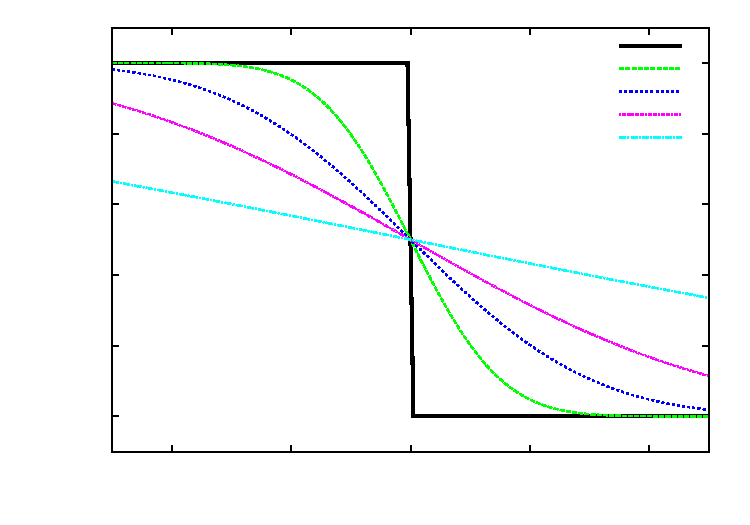
\includegraphics{errorfkt}}%
    \gplfronttext
  \end{picture}%
\endgroup

\caption{Theoretische Erwartungswerte der Diffusionskurven für verschiedene Zeiten mit einem Diffusionskoeffizienten von $D=4\cdot 10^{-10}$m$^2$/s\label{fig:diffkurvetheo}}
\end{figure}
\subsection{Messung 1 und 2}
Um die Diffusionskonstante von Messung 1 zu Bestimmen ist nach der Formel \eqref{eq:c} mit $c=\frac{c_0}{16}$
\begin{align*}
 \frac{1}{16}&=\frac{1}{2}\left(1-\erf{\frac{x}{\sqrt{4Dt}}}\right)\\
 \Rightarrow~ \frac{7}{8}&=\erf{\frac{x}{\sqrt{4Dt}}}
\end{align*}Woraus sich unter Zuhilfenahme von WolframAlpha\textsuperscript{\textregistered}\footnote{www.wolframalpha.com} mit der Umkehrfunktion ergibt
\begin{align*}
 1.0848&\approx \frac{x}{\sqrt{4Dt}}\notag\\
 \Rightarrow~ x^2&=1.0848^2 \cdot 4Dt\notag\\
 x^2&=4.7071\cdot Dt\notag
\end{align*}
Die Steigung, welche in Abb. \ref{fig:M12} zu erkennen ist, ist $m_1=\frac{x^2}{t}$, da der Ort quadratisch gegen die Zeit aufgetragen ist.
\begin{align}
\Rightarrow ~D_1&=\frac{m_1}{4.7071}\label{eq:Dc16}
\end{align}
Analog ergibt sich für Messung 2 mit $c=\frac{c_0}{32}$
\begin{align}
 \frac{15}{16}&=\erf{\frac{x}{\sqrt{4Dt}}}\notag\\
 \Rightarrow~ D_2&=\frac{m_2}{6.9395}\label{eq:Dc32}
\end{align}
Um das $x$ zu berechnen, muss man den Anfangsort $x'(t$=$0)$ von allen gemessenen Werten $x'(t)$ abziehen, damit die Grenzschicht tatsächlich bei $x=0$ liegt.\\  
Die Fehler der beiden Diffusionskonstanten werden mit der Gaußschen Fehlerfortpflanzung bestimmt:
\begin{align*}
 \sigma_{D_1}= \sigma_{m_1}\frac{1}{4.7071}\\
 \sigma_{D_2}= \sigma_{m_2}\frac{1}{4.7071}
\end{align*}
Die Steigung der gefitteten Geraden von Messung 1 aus Abb. \ref{fig:M12} beträgt $(1.34\pm 0.03)\cdot 10^{-9}$m$^2$/s und die von Messung 2 $(2.81\pm 0.07)\cdot 10^{-9}$m$^2$/s.
Daraus ergibt sich nach \eqref{eq:Dc16} und \eqref{eq:Dc32}
\begin{align*}
 D_1&= (2.8\pm 0.1)\cdot 10^{-10}\text{m}^2/\text{s}\\
 D_2&= (4.0\pm 0.2)\cdot 10^{-10}\text{m}^2/\text{s}\\
\end{align*}
Aus dem gewichteten Mittelwert von $D_1$ und $D_2$ ergibt sich 
$$\shadowbox{$D=(3.0\pm 0.1)\cdot 10^{-10}\text{m}^2/\text{s}$}$$

\begin{figure}[!h]
\centering
% GNUPLOT: LaTeX picture with Postscript
\begingroup
  \makeatletter
  \providecommand\color[2][]{%
    \GenericError{(gnuplot) \space\space\space\@spaces}{%
      Package color not loaded in conjunction with
      terminal option `colourtext'%
    }{See the gnuplot documentation for explanation.%
    }{Either use 'blacktext' in gnuplot or load the package
      color.sty in LaTeX.}%
    \renewcommand\color[2][]{}%
  }%
  \providecommand\includegraphics[2][]{%
    \GenericError{(gnuplot) \space\space\space\@spaces}{%
      Package graphicx or graphics not loaded%
    }{See the gnuplot documentation for explanation.%
    }{The gnuplot epslatex terminal needs graphicx.sty or graphics.sty.}%
    \renewcommand\includegraphics[2][]{}%
  }%
  \providecommand\rotatebox[2]{#2}%
  \@ifundefined{ifGPcolor}{%
    \newif\ifGPcolor
    \GPcolortrue
  }{}%
  \@ifundefined{ifGPblacktext}{%
    \newif\ifGPblacktext
    \GPblacktexttrue
  }{}%
  % define a \g@addto@macro without @ in the name:
  \let\gplgaddtomacro\g@addto@macro
  % define empty templates for all commands taking text:
  \gdef\gplbacktext{}%
  \gdef\gplfronttext{}%
  \makeatother
  \ifGPblacktext
    % no textcolor at all
    \def\colorrgb#1{}%
    \def\colorgray#1{}%
  \else
    % gray or color?
    \ifGPcolor
      \def\colorrgb#1{\color[rgb]{#1}}%
      \def\colorgray#1{\color[gray]{#1}}%
      \expandafter\def\csname LTw\endcsname{\color{white}}%
      \expandafter\def\csname LTb\endcsname{\color{black}}%
      \expandafter\def\csname LTa\endcsname{\color{black}}%
      \expandafter\def\csname LT0\endcsname{\color[rgb]{1,0,0}}%
      \expandafter\def\csname LT1\endcsname{\color[rgb]{0,1,0}}%
      \expandafter\def\csname LT2\endcsname{\color[rgb]{0,0,1}}%
      \expandafter\def\csname LT3\endcsname{\color[rgb]{1,0,1}}%
      \expandafter\def\csname LT4\endcsname{\color[rgb]{0,1,1}}%
      \expandafter\def\csname LT5\endcsname{\color[rgb]{1,1,0}}%
      \expandafter\def\csname LT6\endcsname{\color[rgb]{0,0,0}}%
      \expandafter\def\csname LT7\endcsname{\color[rgb]{1,0.3,0}}%
      \expandafter\def\csname LT8\endcsname{\color[rgb]{0.5,0.5,0.5}}%
    \else
      % gray
      \def\colorrgb#1{\color{black}}%
      \def\colorgray#1{\color[gray]{#1}}%
      \expandafter\def\csname LTw\endcsname{\color{white}}%
      \expandafter\def\csname LTb\endcsname{\color{black}}%
      \expandafter\def\csname LTa\endcsname{\color{black}}%
      \expandafter\def\csname LT0\endcsname{\color{black}}%
      \expandafter\def\csname LT1\endcsname{\color{black}}%
      \expandafter\def\csname LT2\endcsname{\color{black}}%
      \expandafter\def\csname LT3\endcsname{\color{black}}%
      \expandafter\def\csname LT4\endcsname{\color{black}}%
      \expandafter\def\csname LT5\endcsname{\color{black}}%
      \expandafter\def\csname LT6\endcsname{\color{black}}%
      \expandafter\def\csname LT7\endcsname{\color{black}}%
      \expandafter\def\csname LT8\endcsname{\color{black}}%
    \fi
  \fi
  \setlength{\unitlength}{0.0500bp}%
  \begin{picture}(7200.00,5040.00)%
    \gplgaddtomacro\gplbacktext{%
      \csname LTb\endcsname%
      \put(1210,704){\makebox(0,0)[r]{\strut{} 0}}%
      \put(1210,1286){\makebox(0,0)[r]{\strut{} 1e-06}}%
      \put(1210,1867){\makebox(0,0)[r]{\strut{} 2e-06}}%
      \put(1210,2449){\makebox(0,0)[r]{\strut{} 3e-06}}%
      \put(1210,3030){\makebox(0,0)[r]{\strut{} 4e-06}}%
      \put(1210,3612){\makebox(0,0)[r]{\strut{} 5e-06}}%
      \put(1210,4193){\makebox(0,0)[r]{\strut{} 6e-06}}%
      \put(1210,4775){\makebox(0,0)[r]{\strut{} 7e-06}}%
      \put(1342,484){\makebox(0,0){\strut{} 0}}%
      \put(1888,484){\makebox(0,0){\strut{} 200}}%
      \put(2434,484){\makebox(0,0){\strut{} 400}}%
      \put(2980,484){\makebox(0,0){\strut{} 600}}%
      \put(3526,484){\makebox(0,0){\strut{} 800}}%
      \put(4073,484){\makebox(0,0){\strut{} 1000}}%
      \put(4619,484){\makebox(0,0){\strut{} 1200}}%
      \put(5165,484){\makebox(0,0){\strut{} 1400}}%
      \put(5711,484){\makebox(0,0){\strut{} 1600}}%
      \put(6257,484){\makebox(0,0){\strut{} 1800}}%
      \put(6803,484){\makebox(0,0){\strut{} 2000}}%
      \put(176,2739){\rotatebox{-270}{\makebox(0,0){\strut{}Höhe im Quadrat [m$^2$]}}}%
      \put(4072,154){\makebox(0,0){\strut{}Zeit [s]}}%
    }%
    \gplgaddtomacro\gplfronttext{%
      \csname LTb\endcsname%
      \put(3190,4602){\makebox(0,0)[r]{\strut{}Messung 1}}%
      \csname LTb\endcsname%
      \put(3190,4382){\makebox(0,0)[r]{\strut{}Fit Messung 1}}%
      \csname LTb\endcsname%
      \put(3190,4162){\makebox(0,0)[r]{\strut{}Messung 2}}%
      \csname LTb\endcsname%
      \put(3190,3942){\makebox(0,0)[r]{\strut{}Fit Messung 2}}%
    }%
    \gplbacktext
    \put(0,0){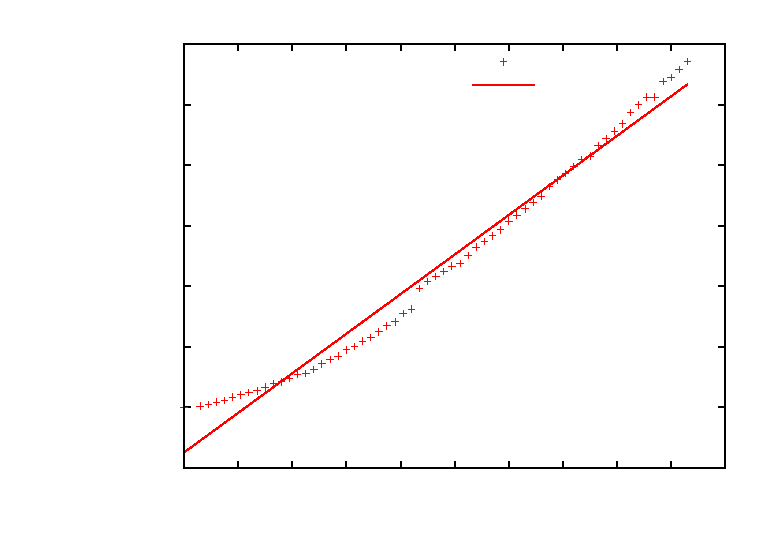
\includegraphics{v1ges}}%
    \gplfronttext
  \end{picture}%
\endgroup

\caption{Messung 1 und 2: Auftragung der Höhe der Konzentration $c_0/16$ und $c_0/32$ im Quadrat gegen die Zeit mit dem zugehörigen Fit\label{fig:M12}}
\end{figure}

\subsection{Messung 3 und 4}
\begin{figure}[h!]
 \centering
 % GNUPLOT: LaTeX picture with Postscript
\begingroup
  \makeatletter
  \providecommand\color[2][]{%
    \GenericError{(gnuplot) \space\space\space\@spaces}{%
      Package color not loaded in conjunction with
      terminal option `colourtext'%
    }{See the gnuplot documentation for explanation.%
    }{Either use 'blacktext' in gnuplot or load the package
      color.sty in LaTeX.}%
    \renewcommand\color[2][]{}%
  }%
  \providecommand\includegraphics[2][]{%
    \GenericError{(gnuplot) \space\space\space\@spaces}{%
      Package graphicx or graphics not loaded%
    }{See the gnuplot documentation for explanation.%
    }{The gnuplot epslatex terminal needs graphicx.sty or graphics.sty.}%
    \renewcommand\includegraphics[2][]{}%
  }%
  \providecommand\rotatebox[2]{#2}%
  \@ifundefined{ifGPcolor}{%
    \newif\ifGPcolor
    \GPcolortrue
  }{}%
  \@ifundefined{ifGPblacktext}{%
    \newif\ifGPblacktext
    \GPblacktexttrue
  }{}%
  % define a \g@addto@macro without @ in the name:
  \let\gplgaddtomacro\g@addto@macro
  % define empty templates for all commands taking text:
  \gdef\gplbacktext{}%
  \gdef\gplfronttext{}%
  \makeatother
  \ifGPblacktext
    % no textcolor at all
    \def\colorrgb#1{}%
    \def\colorgray#1{}%
  \else
    % gray or color?
    \ifGPcolor
      \def\colorrgb#1{\color[rgb]{#1}}%
      \def\colorgray#1{\color[gray]{#1}}%
      \expandafter\def\csname LTw\endcsname{\color{white}}%
      \expandafter\def\csname LTb\endcsname{\color{black}}%
      \expandafter\def\csname LTa\endcsname{\color{black}}%
      \expandafter\def\csname LT0\endcsname{\color[rgb]{1,0,0}}%
      \expandafter\def\csname LT1\endcsname{\color[rgb]{0,1,0}}%
      \expandafter\def\csname LT2\endcsname{\color[rgb]{0,0,1}}%
      \expandafter\def\csname LT3\endcsname{\color[rgb]{1,0,1}}%
      \expandafter\def\csname LT4\endcsname{\color[rgb]{0,1,1}}%
      \expandafter\def\csname LT5\endcsname{\color[rgb]{1,1,0}}%
      \expandafter\def\csname LT6\endcsname{\color[rgb]{0,0,0}}%
      \expandafter\def\csname LT7\endcsname{\color[rgb]{1,0.3,0}}%
      \expandafter\def\csname LT8\endcsname{\color[rgb]{0.5,0.5,0.5}}%
    \else
      % gray
      \def\colorrgb#1{\color{black}}%
      \def\colorgray#1{\color[gray]{#1}}%
      \expandafter\def\csname LTw\endcsname{\color{white}}%
      \expandafter\def\csname LTb\endcsname{\color{black}}%
      \expandafter\def\csname LTa\endcsname{\color{black}}%
      \expandafter\def\csname LT0\endcsname{\color{black}}%
      \expandafter\def\csname LT1\endcsname{\color{black}}%
      \expandafter\def\csname LT2\endcsname{\color{black}}%
      \expandafter\def\csname LT3\endcsname{\color{black}}%
      \expandafter\def\csname LT4\endcsname{\color{black}}%
      \expandafter\def\csname LT5\endcsname{\color{black}}%
      \expandafter\def\csname LT6\endcsname{\color{black}}%
      \expandafter\def\csname LT7\endcsname{\color{black}}%
      \expandafter\def\csname LT8\endcsname{\color{black}}%
    \fi
  \fi
  \setlength{\unitlength}{0.0500bp}%
  \begin{picture}(7200.00,5040.00)%
    \gplgaddtomacro\gplbacktext{%
      \csname LTb\endcsname%
      \put(946,704){\makebox(0,0)[r]{\strut{} 0}}%
      \put(946,1383){\makebox(0,0)[r]{\strut{} 0.1}}%
      \put(946,2061){\makebox(0,0)[r]{\strut{} 0.2}}%
      \put(946,2740){\makebox(0,0)[r]{\strut{} 0.3}}%
      \put(946,3418){\makebox(0,0)[r]{\strut{} 0.4}}%
      \put(946,4097){\makebox(0,0)[r]{\strut{} 0.5}}%
      \put(946,4775){\makebox(0,0)[r]{\strut{} 0.6}}%
      \put(1263,484){\makebox(0,0){\strut{} 0}}%
      \put(2186,484){\makebox(0,0){\strut{} 1}}%
      \put(3109,484){\makebox(0,0){\strut{} 2}}%
      \put(4033,484){\makebox(0,0){\strut{} 3}}%
      \put(4956,484){\makebox(0,0){\strut{} 4}}%
      \put(5880,484){\makebox(0,0){\strut{} 5}}%
      \put(6803,484){\makebox(0,0){\strut{} 6}}%
      \put(176,2739){\rotatebox{-270}{\makebox(0,0){\strut{}c/c$_0$}}}%
      \put(3940,154){\makebox(0,0){\strut{}x [mm]}}%
    }%
    \gplgaddtomacro\gplfronttext{%
      \csname LTb\endcsname%
      \put(5816,4602){\makebox(0,0)[r]{\strut{}Messwerte}}%
      \csname LTb\endcsname%
      \put(5816,4382){\makebox(0,0)[r]{\strut{}Theorie für t = 41 min}}%
    }%
    \gplbacktext
    \put(0,0){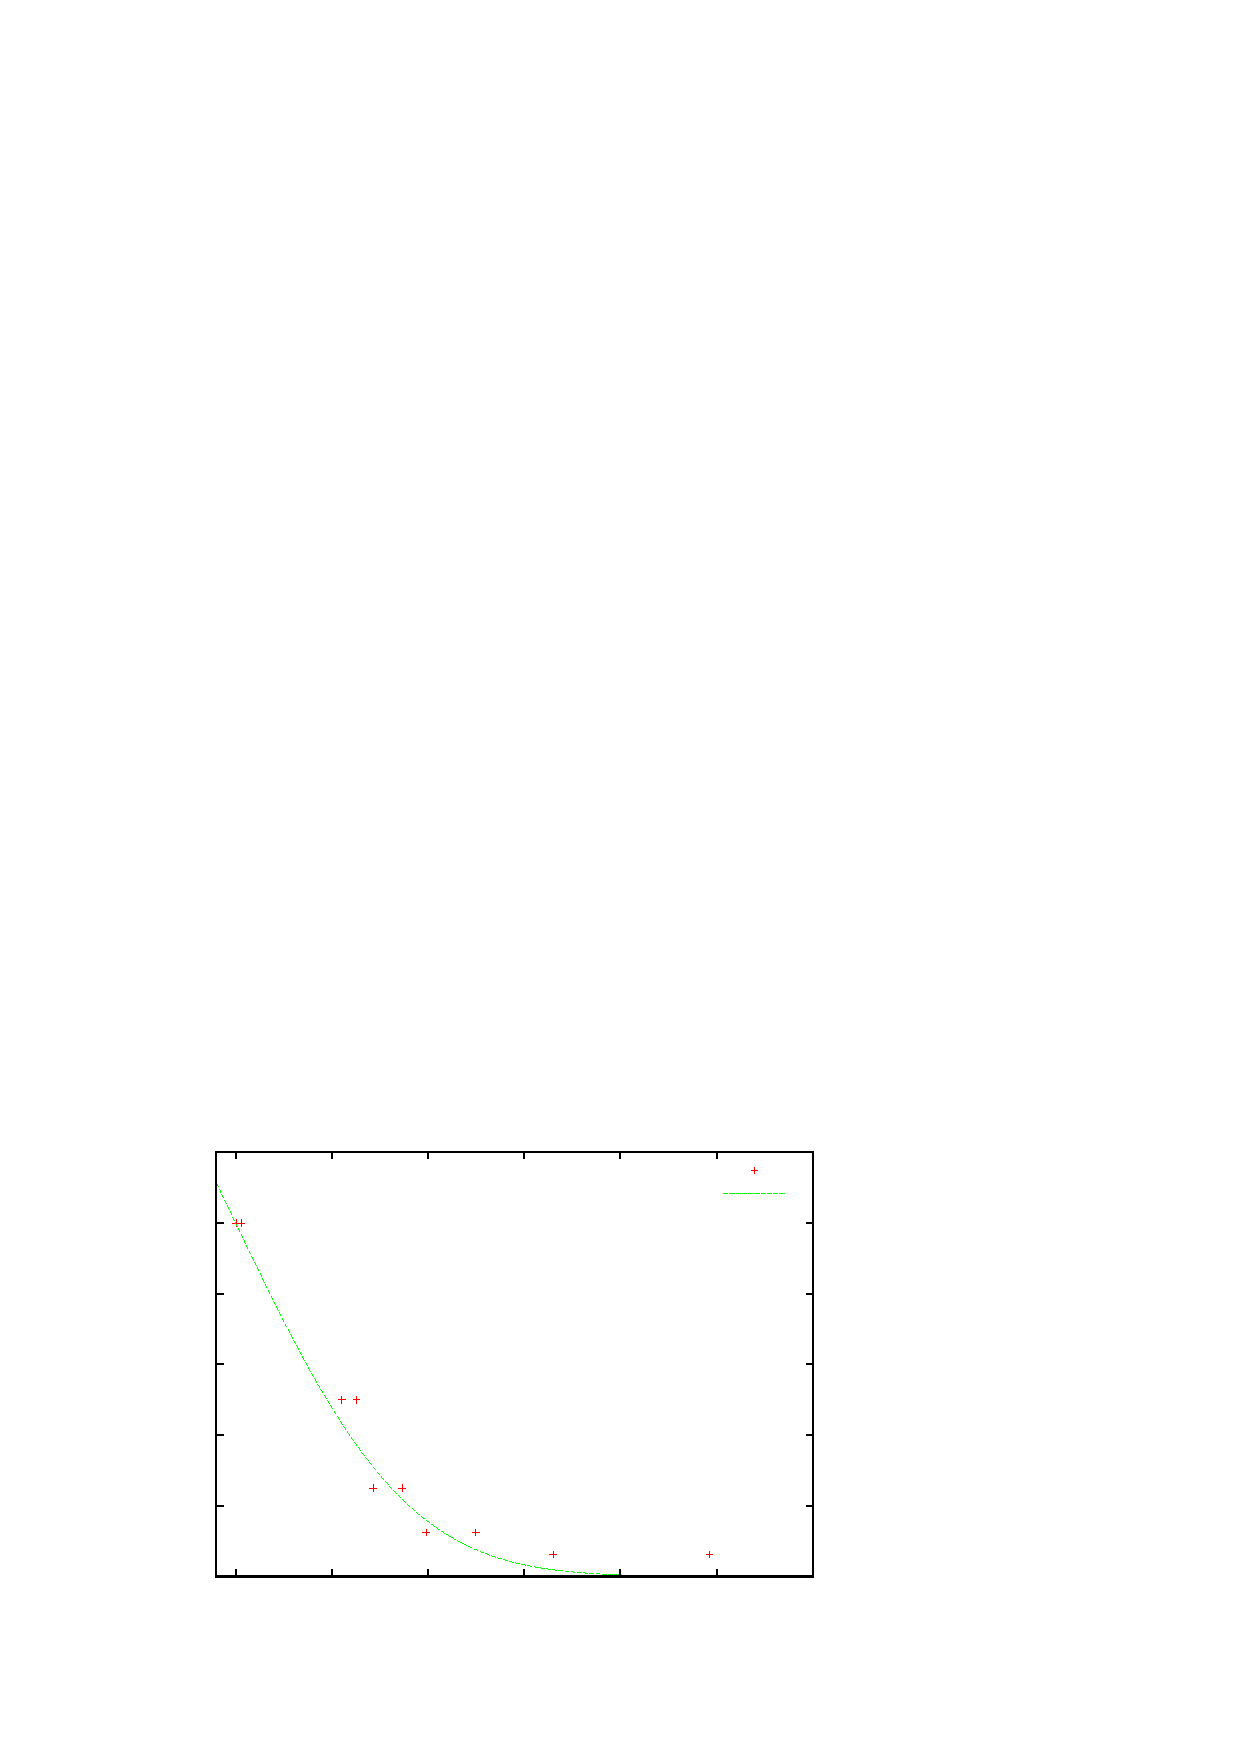
\includegraphics{profiel1}}%
    \gplfronttext
  \end{picture}%
\endgroup

 \caption{Messung von Versuch 3 zusammen mit dem theoretischen Wert für die durchschnittliche Zeit der Messung\label{fig:m3}}
\end{figure}
\begin{figure}[h!]
 \centering
 % GNUPLOT: LaTeX picture with Postscript
\begingroup
  \makeatletter
  \providecommand\color[2][]{%
    \GenericError{(gnuplot) \space\space\space\@spaces}{%
      Package color not loaded in conjunction with
      terminal option `colourtext'%
    }{See the gnuplot documentation for explanation.%
    }{Either use 'blacktext' in gnuplot or load the package
      color.sty in LaTeX.}%
    \renewcommand\color[2][]{}%
  }%
  \providecommand\includegraphics[2][]{%
    \GenericError{(gnuplot) \space\space\space\@spaces}{%
      Package graphicx or graphics not loaded%
    }{See the gnuplot documentation for explanation.%
    }{The gnuplot epslatex terminal needs graphicx.sty or graphics.sty.}%
    \renewcommand\includegraphics[2][]{}%
  }%
  \providecommand\rotatebox[2]{#2}%
  \@ifundefined{ifGPcolor}{%
    \newif\ifGPcolor
    \GPcolortrue
  }{}%
  \@ifundefined{ifGPblacktext}{%
    \newif\ifGPblacktext
    \GPblacktexttrue
  }{}%
  % define a \g@addto@macro without @ in the name:
  \let\gplgaddtomacro\g@addto@macro
  % define empty templates for all commands taking text:
  \gdef\gplbacktext{}%
  \gdef\gplfronttext{}%
  \makeatother
  \ifGPblacktext
    % no textcolor at all
    \def\colorrgb#1{}%
    \def\colorgray#1{}%
  \else
    % gray or color?
    \ifGPcolor
      \def\colorrgb#1{\color[rgb]{#1}}%
      \def\colorgray#1{\color[gray]{#1}}%
      \expandafter\def\csname LTw\endcsname{\color{white}}%
      \expandafter\def\csname LTb\endcsname{\color{black}}%
      \expandafter\def\csname LTa\endcsname{\color{black}}%
      \expandafter\def\csname LT0\endcsname{\color[rgb]{1,0,0}}%
      \expandafter\def\csname LT1\endcsname{\color[rgb]{0,1,0}}%
      \expandafter\def\csname LT2\endcsname{\color[rgb]{0,0,1}}%
      \expandafter\def\csname LT3\endcsname{\color[rgb]{1,0,1}}%
      \expandafter\def\csname LT4\endcsname{\color[rgb]{0,1,1}}%
      \expandafter\def\csname LT5\endcsname{\color[rgb]{1,1,0}}%
      \expandafter\def\csname LT6\endcsname{\color[rgb]{0,0,0}}%
      \expandafter\def\csname LT7\endcsname{\color[rgb]{1,0.3,0}}%
      \expandafter\def\csname LT8\endcsname{\color[rgb]{0.5,0.5,0.5}}%
    \else
      % gray
      \def\colorrgb#1{\color{black}}%
      \def\colorgray#1{\color[gray]{#1}}%
      \expandafter\def\csname LTw\endcsname{\color{white}}%
      \expandafter\def\csname LTb\endcsname{\color{black}}%
      \expandafter\def\csname LTa\endcsname{\color{black}}%
      \expandafter\def\csname LT0\endcsname{\color{black}}%
      \expandafter\def\csname LT1\endcsname{\color{black}}%
      \expandafter\def\csname LT2\endcsname{\color{black}}%
      \expandafter\def\csname LT3\endcsname{\color{black}}%
      \expandafter\def\csname LT4\endcsname{\color{black}}%
      \expandafter\def\csname LT5\endcsname{\color{black}}%
      \expandafter\def\csname LT6\endcsname{\color{black}}%
      \expandafter\def\csname LT7\endcsname{\color{black}}%
      \expandafter\def\csname LT8\endcsname{\color{black}}%
    \fi
  \fi
  \setlength{\unitlength}{0.0500bp}%
  \begin{picture}(7200.00,5040.00)%
    \gplgaddtomacro\gplbacktext{%
      \csname LTb\endcsname%
      \put(1078,704){\makebox(0,0)[r]{\strut{} 0}}%
      \put(1078,1074){\makebox(0,0)[r]{\strut{} 0.05}}%
      \put(1078,1444){\makebox(0,0)[r]{\strut{} 0.1}}%
      \put(1078,1814){\makebox(0,0)[r]{\strut{} 0.15}}%
      \put(1078,2184){\makebox(0,0)[r]{\strut{} 0.2}}%
      \put(1078,2554){\makebox(0,0)[r]{\strut{} 0.25}}%
      \put(1078,2925){\makebox(0,0)[r]{\strut{} 0.3}}%
      \put(1078,3295){\makebox(0,0)[r]{\strut{} 0.35}}%
      \put(1078,3665){\makebox(0,0)[r]{\strut{} 0.4}}%
      \put(1078,4035){\makebox(0,0)[r]{\strut{} 0.45}}%
      \put(1078,4405){\makebox(0,0)[r]{\strut{} 0.5}}%
      \put(1078,4775){\makebox(0,0)[r]{\strut{} 0.55}}%
      \put(1346,484){\makebox(0,0){\strut{} 0}}%
      \put(2028,484){\makebox(0,0){\strut{} 0.0005}}%
      \put(2711,484){\makebox(0,0){\strut{} 0.001}}%
      \put(3393,484){\makebox(0,0){\strut{} 0.0015}}%
      \put(4075,484){\makebox(0,0){\strut{} 0.002}}%
      \put(4757,484){\makebox(0,0){\strut{} 0.0025}}%
      \put(5439,484){\makebox(0,0){\strut{} 0.003}}%
      \put(6121,484){\makebox(0,0){\strut{} 0.0035}}%
      \put(6803,484){\makebox(0,0){\strut{} 0.004}}%
      \put(176,2739){\rotatebox{-270}{\makebox(0,0){\strut{}$\frac{\text{c}}{\text{c}_0}$}}}%
      \put(4006,154){\makebox(0,0){\strut{}x [m]}}%
    }%
    \gplgaddtomacro\gplfronttext{%
      \csname LTb\endcsname%
      \put(5816,4602){\makebox(0,0)[r]{\strut{}Messwerte}}%
      \csname LTb\endcsname%
      \put(5816,4382){\makebox(0,0)[r]{\strut{}Theorie für t = 96 min}}%
    }%
    \gplbacktext
    \put(0,0){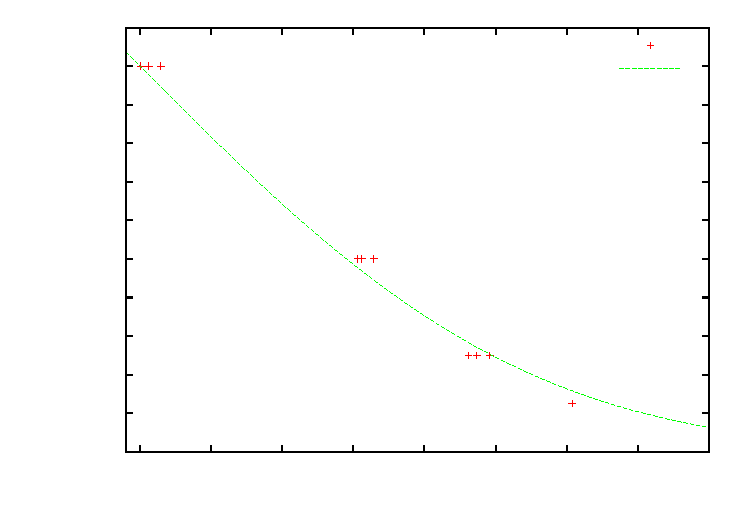
\includegraphics{profiel2}}%
    \gplfronttext
  \end{picture}%
\endgroup

 \caption{Messung von Versuch 4 zusammen mit dem theoretischen Wert für die durchschnittliche Zeit der Messung\label{fig:m4}}
\end{figure}
Bei Messung 3 und 4 wurde in einer möglichst kurzen Zeit der Konzentrationsverlauf der beiden Küvetten gemessen.
Für die beiden Messungen haben wir 15min und 17min benötigt.
Dies ist relativ lange, da wir Messung 3 schon 34min nach Überschichtung begannen.
Die Ergebnisse haben wir in Abb. \ref{fig:m3} und \ref{fig:m4} zusammen mit der theoretischen Erwartung für die jeweilige mittlere Zeit aufgetragen.

\newpage
\section{Diskussion}
\label{sec:diskussion}
\subsection{Messung 1 und 2}
Die mithilfe des gewichteten Mittelwertes bestimmte Diffusionskonstante beträgt $=(3.0\pm 0.1)\cdot 10^{-10}\text{m}^2/\text{s}$.
Dies ist 25\% kleiner, als der im Praktikumshandbuch oder im \cite{LP} vorgeschlagene Wert von $D_{Handbuch}=4\cdot 10^{-10}\text{m}^2/\text{s}$.
Der Wert $D_1$ entspricht hierbei genau diesem Wert.
Die Steigung des Fits der ersten Messung war zu gering.
Hier könnte ein verschmutzter Graufilter die Ursache gewesen sein, welcher uns für die Auswertung eine niedrigere, als die eigentlich gemessene Konzentration, zu haben schien.
Eine weitere Fehlerquelle ist die Lampe, welche die Küvette zusammen mit den darin enthaltenen Flüssigkeiten mit der Zeit erhitzt.
Dies schien besonders bei der zweiten Messung einen Einfluss gehabt zu haben, da der Plot offenbart, dass die Steigung im Verlaufe der Zeit steigt.\\
Ein weiterer möglicher Fehler war, dass wir zur Umrechnung von $x$ aus unseren gemessenen Werten davon ausgegangen sind, dass wir sofort nach der Überschichtung mit der Messung begonnen haben.
Die ist in der Realität jedoch nicht umsetzbar, zumal es während des Befüllens schon zu einer Vermischung der beiden Flüssigkeiten kommt.\\

Trägt man die Messwerte von Messung 1 in einem Diagramm auf, so ist offensichtlich zwischen 14min und 14.5min ein Sprung in den Werten.
Dieser ist durch einen Stoß an den Tisch zu erklären, welcher die Vermischung der Flüssigkeiten in dem Moment extrem beschleunigt hat.

\subsection{Messung 3 und 4}
Bei der Betrachtung der Graphen fällt auf, dass (vor allem bei Messung $4$ in Abb. \ref{fig:m4}) die einzelnen Gruppen bestimmter Konzentrationen zwar relativ eng beieinander, jedoch selten auf beiden Seiten der theoretischen Werte für die durchschnittliche Zeit liegen.
Dies deutet auf unsaubere Filter (insbesondere $c_0/2$ und $c_0/4$, welche in beiden Messungen rechts der Theorie liegen) hin, welche ihre jeweiligen Messungen verfälscht haben.
Die wohl größte Fehlerquelle bei diesen Versuchen war unser Anspruch, möglichst genau und ohne die Probe zu stark zu bewegen zu messen.
Dadurch haben wir extrem lange für diese Messung benötigt.
Man sollte hierbei einen Mittelweg finden.

\subsection{Allgemeine Verbesserungsvorschläge}
Man sollte die Filter vor jeder Nutzung auf Schmutzreste überprüfen.
Insbesondere sollte man sie nur am Rand anfassen, damit keine Fettreste zurückbleiben.\\
Auch könnte man die Entfernung der Lampe von der Küvette etwas erhöhen, was die Erwärmung der Flüssigkeiten verzögern würde.
Allerdings würde so auch das vom Photosensor empfangene Licht geringer werden, was wiederum Fehler hervorrufen könnte.
Desweiteren ist darauf zu achten, das Licht im Raum möglichst stark zu dimmen, da uns auffiel, dass das Öffnen der Tür und damit ein Lichteinfall unser Ampèremeter hat ausschlagen lassen.
Auch ist es wichtig, nicht zu wenig Wasser in die Küvette zu füllen, da insbesondere bei Messung 4 man sonst schnell an die Grenzen des Statives kommt. 
\section{Anhang}
\bibliography{literatur}
\bibliographystyle{babalpha}
%\bibliographystyle{alpha}
\end{document}
